\documentclass[aps,prx,preprint,floatfix,superscriptaddress]{revtex4-2}
\usepackage[T1]{fontenc}
\usepackage[utf8]{inputenc}
\usepackage{microtype}
\usepackage{amssymb,mathtools}
\usepackage{booktabs}
\usepackage{array}
\usepackage{longtable}
\usepackage{graphicx}
\usepackage{xcolor}
\usepackage{hyperref}
\hypersetup{hidelinks}

\makeatletter
\let\switch@array\relax
\makeatother

\newcommand{\DataNumber}[2]{#2}
% Generated by scripts/build_all_tables.py; do not edit.
\newcommand{\TradeoffRuns}{\DataNumber{w3-cells}{592}}
\newcommand{\MatchedCells}{\DataNumber{w4-cells}{1,080}}
\newcommand{\MatchedCompleted}{\DataNumber{w4-completed}{1,065}}
\newcommand{\MatchedPredicateErrors}{\DataNumber{w4-predicate-errors}{15}}
\newcommand{\ExternalCells}{\DataNumber{w5-cells}{1,728}}
\newcommand{\ExternalCompleted}{\DataNumber{w5-completed}{1,695}}
\newcommand{\ExternalPredicateErrors}{\DataNumber{w5-predicate-errors}{33}}
\newcommand{\CertificateMutationCases}{\DataNumber{w6-mutations}{56}}
\newcommand{\CertificateFalseAccepts}{\DataNumber{w6-false-accepts}{0}}
\newcommand{\CertificateCrosscheckCases}{\DataNumber{w6-crosschecks}{12}}
\newcommand{\QRECells}{\DataNumber{w7-cells}{288}}
\newcommand{\QREMaterializeSpacetimeRatio}{\DataNumber{w7-spacetime-ratio}{2814}}
\newcommand{\NaturalCells}{\DataNumber{w8-cells}{21,060}}
\newcommand{\NaturalStableFamilies}{\DataNumber{w8-stable-families}{5}}
\newcommand{\NaturalNegativeRegressions}{\DataNumber{w8-negative-regressions}{0}}
\newcommand{\PresetGateEffect}{\DataNumber{w8-preset-effect}{364.9}}
\newcommand{\PresetGateEffectLow}{\DataNumber{w8-preset-effect-low}{349.8}}
\newcommand{\PresetGateEffectHigh}{\DataNumber{w8-preset-effect-high}{380.5}}
\newcommand{\UnifiedRows}{\DataNumber{w9-unified-rows}{24,748}}
\newcommand{\UnifiedPredicateErrors}{\DataNumber{w9-predicate-errors}{48}}
\newcommand{\CleanTheoryTests}{\DataNumber{w9-clean-theorem-tests}{9}}
\newcommand{\CleanGridPairs}{\DataNumber{w9-clean-grid-pairs}{17}}


\begin{document}

\title{Supplemental Material for\\
``Representation as a Computational Resource in Quantum Compilation:\\
Approximate Recoverability Tradeoffs and Model-Specific\\
Fault-Tolerant Consequences''}
\author{Jinze Yang}
\affiliation{School of Physics, Xidian University, Xi'an 710071, China}
\author{Yangyang Li}
\affiliation{School of Artificial Intelligence, Xidian University, Xi'an 710071, China}
\author{Xiu-Hao Deng}
\affiliation{Shenzhen International Quantum Academy, Shenzhen 518048, China}
\date{August 3, 2026}
\maketitle

\section{Scope and evidence policy}
\label{supp:scope}

This document contains expanded experimental protocols, negative results,
status accounting, a historical/stress-result registry, and data provenance
for the full-length main manuscript.  The headline proof and the earlier
application appendices remain in the active main manuscript so that their
assumptions, constructions, and scope are visible together.  Historical files
are retained for auditability but are not promoted to canonical W3--W9
evidence unless they appear in
\path{data/manifest.yaml}.

Only \texttt{completed\_valid} or a campaign-specific \texttt{completed}
paired with a passing independent certificate is an accepted quality outcome.
\texttt{timeout}, \texttt{memory\_error}, \texttt{unsupported},
\texttt{predicate\_error}, \texttt{correctness\_failure}, and
\texttt{numerical\_inconclusive} remain separate categories.  A failed or
unsupported cell is never assigned an infinite, zero, or best-available
metric.

\begin{table}[h]
\caption{Canonical campaign inventory.  Counts are generated from registered
frozen sources; status-only rows remain in their source tables.}
\label{supp:tab:campaigns}
\centering
\begin{tabular}{lll}
\toprule
Package & Canonical cells & Audit status\\
\midrule
W3 tradeoff traces & \TradeoffRuns & all theorem diagnostics pass\\
W4 matched representations & \MatchedCells & \MatchedCompleted\ completed; \MatchedPredicateErrors\ predicate errors\\
W5 external baselines & \ExternalCells & \ExternalCompleted\ completed; \ExternalPredicateErrors\ predicate errors\\
W6 certificate audit & \CertificateMutationCases\ mutations & \CertificateFalseAccepts\ false accepts\\
W7 fixed-error QRE & \QRECells & all completed-valid\\
W8 natural factorial & \NaturalCells & all completed-valid\\
W9 normalized index & \UnifiedRows & unique complete keys\\
\bottomrule
\end{tabular}
\end{table}

\section{Instrumented commitment--state--IR campaign}
\label{supp:w3}

The W3 reference suite is a collection of formal-model objects, not wrappers
around production compilers.  The event schema records input position, pass,
control/store/window bytes, parameter bytes, serialized live-IR bytes,
committed output delta and total, RSS, and wall time.  The theorem coordinate
$S$ is computed from the complete serialized cut state.  RSS is an ancillary
operational measurement and is never used as a proof surrogate.

\begin{table}[h]
\caption{Reference compiler behaviors.  Memory percentages refer to the
payload portion of the full aggregate vector; framing remains charged.}
\label{supp:tab:w3-compilers}
\centering
\begin{tabular}{lll}
\toprule
Compiler & Aggregate memory & Commitment policy\\
\midrule
Echo & none & append each update in stream order\\
Full aggregation & full & retain vector, emit canonical aggregate\\
Hybrid-25 & 25\% & aggregate public block, pass through remainder\\
Hybrid-50 & 50\% & aggregate public block, pass through remainder\\
Hybrid-75 & 75\% & aggregate public block, pass through remainder\\
IR materializing & full plus IR & retain explicit materialized stream\\
\bottomrule
\end{tabular}
\end{table}

The grid crosses $m$, update rounds, $K$, separation margin, forward passes,
memory cap, schedule, and seed.  Every run has a per-run manifest and event
log.  The aggregate file \path{data/frozen/tradeoff_summary.csv} reports both
the exact transcript residual and the state-cap envelope residual.  The frozen
anomaly table is empty; this is reported as an observed campaign fact, not
substituted for the theorem.

\begin{figure}[h]
\centering
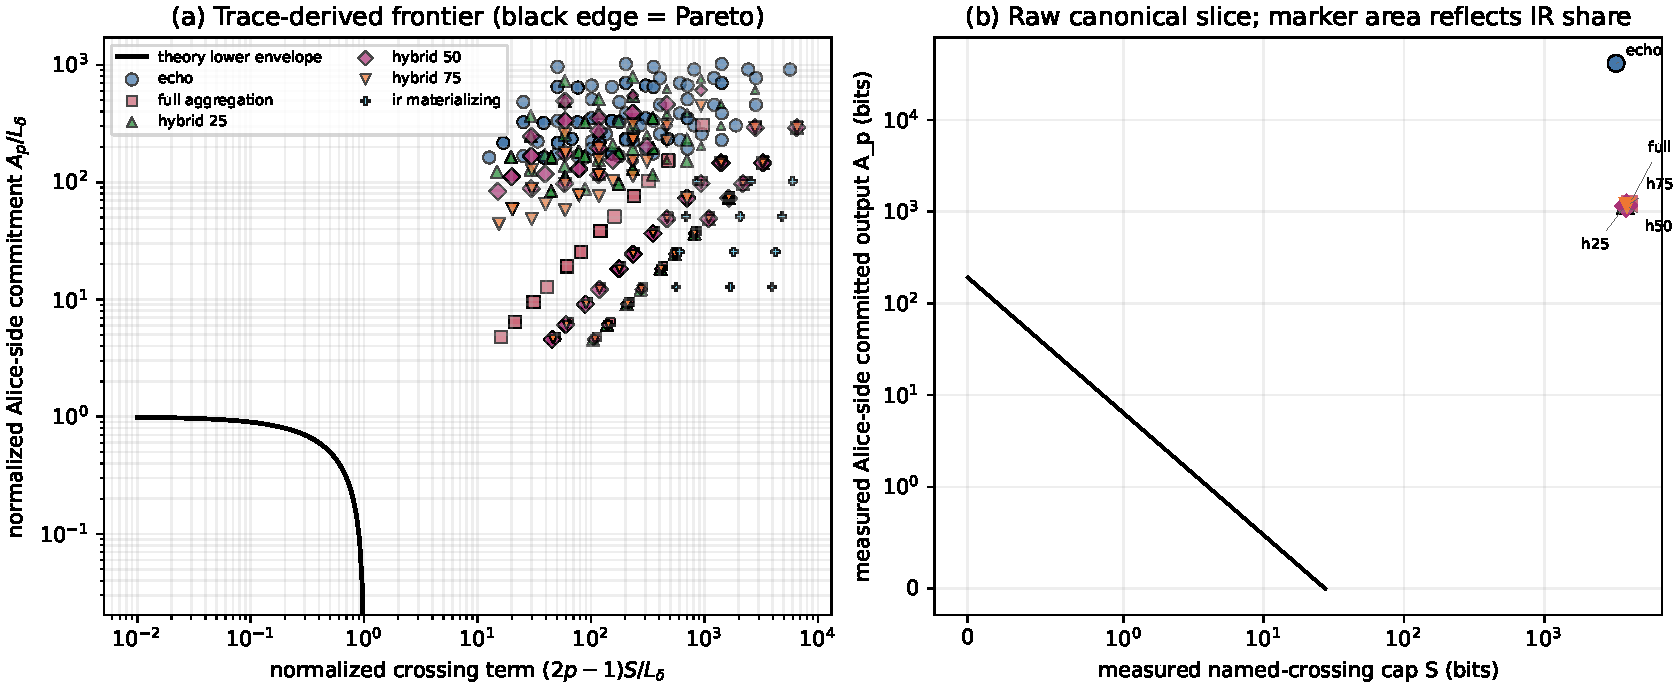
\includegraphics[width=0.92\textwidth]{../../figures/measured_tradeoff_frontier.pdf}
\caption{Complete event-traced W3 surface.}
\label{supp:fig:w3}
\end{figure}

\section{Matched representations and external semantic baselines}
\label{supp:w4w5}

For each target the generator creates semantic aggregate, contiguous flat,
round-robin flat, random commuting order, masked-share/update stream, locally
folded flat, QASM bridge, TKET bridge, and ZX bridge forms.  The representation
record freezes its identifier, seed, generation parameters, serialized sizes,
input certificate, and content hashes.  Compilers see the same target basis,
hardware abstraction, timeout, memory cap, and certificate.

The five W4 reference compilers are echo/pass-through, full aggregation,
memory-capped hybrid, local Qiskit, and the authors' exact phase-table
reference.  W5 then applies eight frozen configurations: native and unified
forms of the authors reference, Qiskit level-three local optimization, TKET
PauliSimp, and PyZX full-reduce.  Native-to-unified bridge deltas are measured
before certificate comparison.  A semantic-capable external output is grouped
with the semantic side even when it is more compact than the authors output.

\begin{figure}[h]
\centering
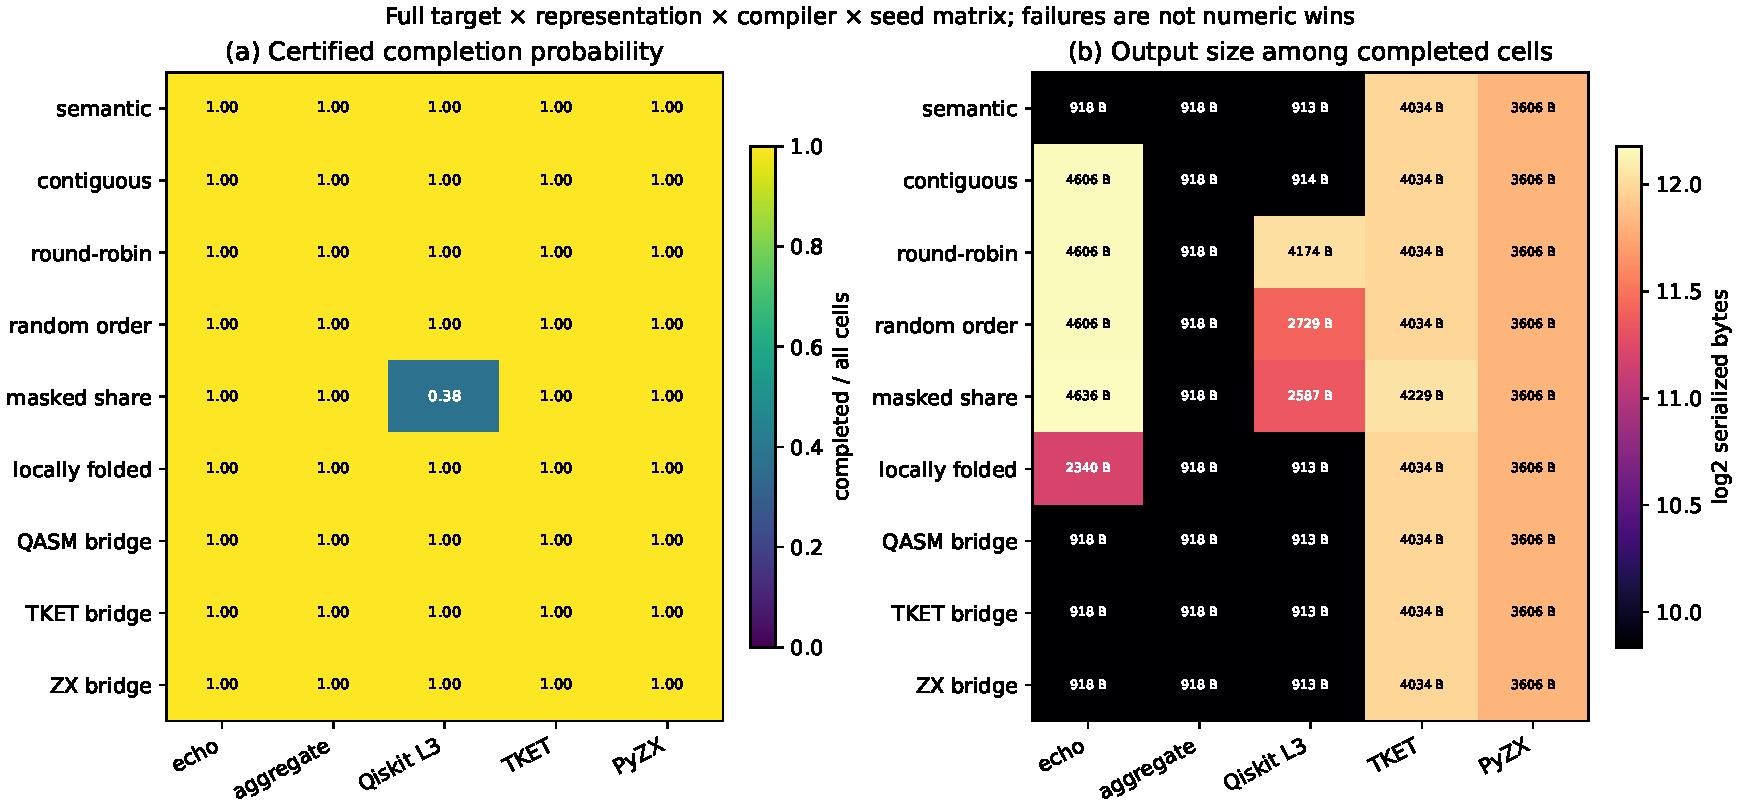
\includegraphics[width=0.92\textwidth]{../../figures/representation_compiler_interaction.pdf}
\caption{Full representation--compiler interaction summary; completion
probability is separated from completed-cell metrics.}
\label{supp:fig:w4}
\end{figure}

The fifteen W4 predicate errors and thirty-three W5 predicate errors are
retained in the canonical parquet files.  They arise when an output lies
outside the declared certificate predicate; they are neither correctness
failures nor wins.  No completed output bypasses the independent certificate.

\section{Correctness certificate adversarial audit}
\label{supp:w6}

The exact checker accepts commuting Pauli rotations in a tracked Clifford
frame with rational-$\pi$ and declared formal-symbol coefficients.  It moves a
Pauli sign into the coefficient, reduces the rational-$\pi$ component modulo
$2\pi$, discards global phase, merges equal supports, and sorts addressed
records deterministically.  Equality of the canonical frame and rotation
records implies projective unitary equality in the stated domain.

The mutation suite changes one angle, sign, support bit, qubit permutation,
Clifford frame, deleted gate, or duplicated gate.  Dense matrices through six
qubits form an independent cross-check.  The frozen result contains
\CertificateMutationCases\ mutations, \CertificateCrosscheckCases\ accepted
and rejected cross-check cases, \CertificateFalseAccepts\ false accepts, and
no dense/symbolic disagreement.  Floating-only parameters, unlisted gates, and
noncommuting extracted networks are explicitly outside the acceptance domain.

\section{Fixed-total-error QRE details}
\label{supp:w7}

The budget schema requires
\begin{equation}
 \epsilon_{\rm alg}+\epsilon_{\rm synth}+\epsilon_{\rm logical}
 \leq\epsilon_{\rm total}.
\end{equation}
The campaign uses the same fractional split in every pipeline and reallocates
per-rotation synthesis accuracy after compilation.  Equal-decimal allocation
and a cost-optimized discrete allocation are both retained.  The deterministic
staq grid-synthesis executable runs with checking enabled; an angle cache is
keyed by the exact angle/precision pair and records every use.

\begin{table}[h]
\caption{QRE factorial controls.}
\label{supp:tab:qre-grid}
\centering
\begin{tabular}{ll}
\toprule
Dimension & Frozen levels\\
\midrule
Total error & $10^{-3},10^{-6},10^{-9}$\\
Allocation & equal decimal; cost optimized\\
QEC assumptions & conservative; improved surface-code profiles\\
Factory parallelism & serialized, low, medium, high Pareto points\\
Pipelines & semantic-first; materialize-first; external TKET PauliSimp\\
Outputs & rotations, $T$, qubits, factories, cycles, runtime, spacetime\\
\bottomrule
\end{tabular}
\end{table}

\begin{figure}[h]
\centering
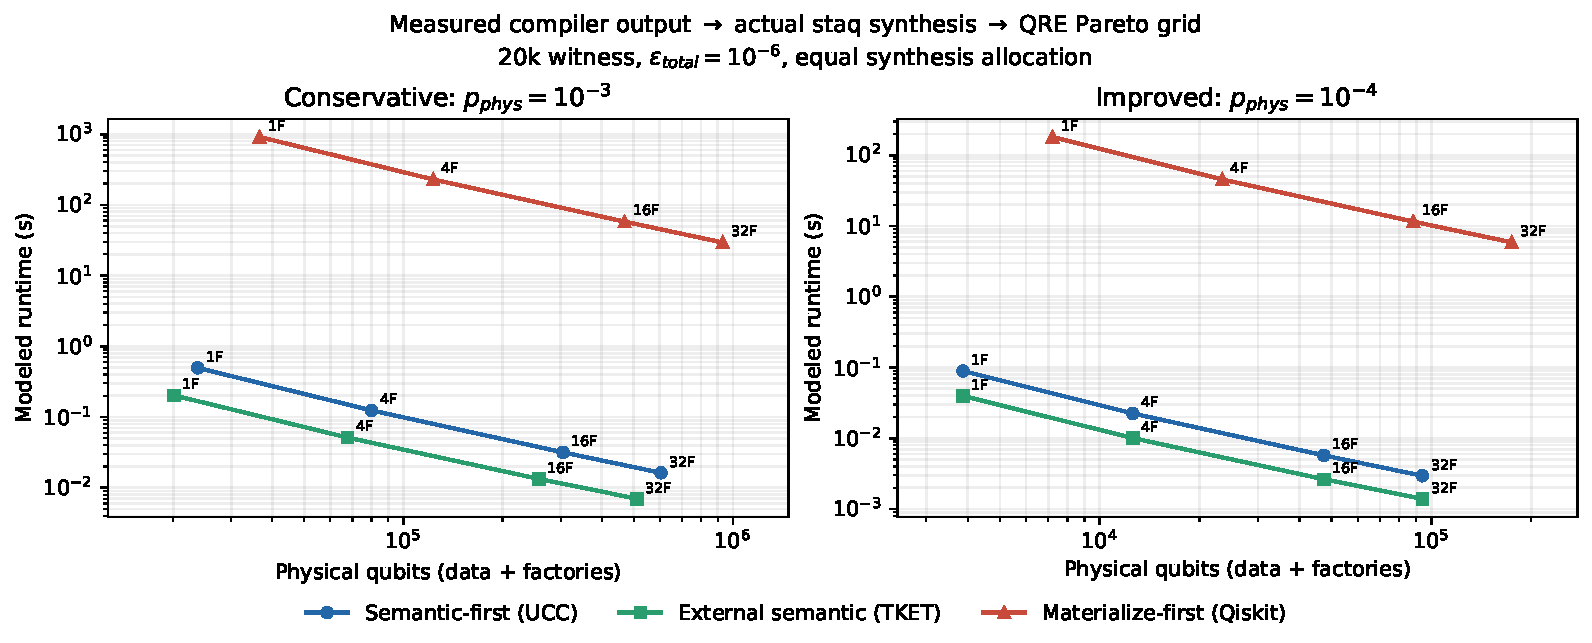
\includegraphics[width=0.48\textwidth]{../../figures/qre_pareto.pdf}\hfill
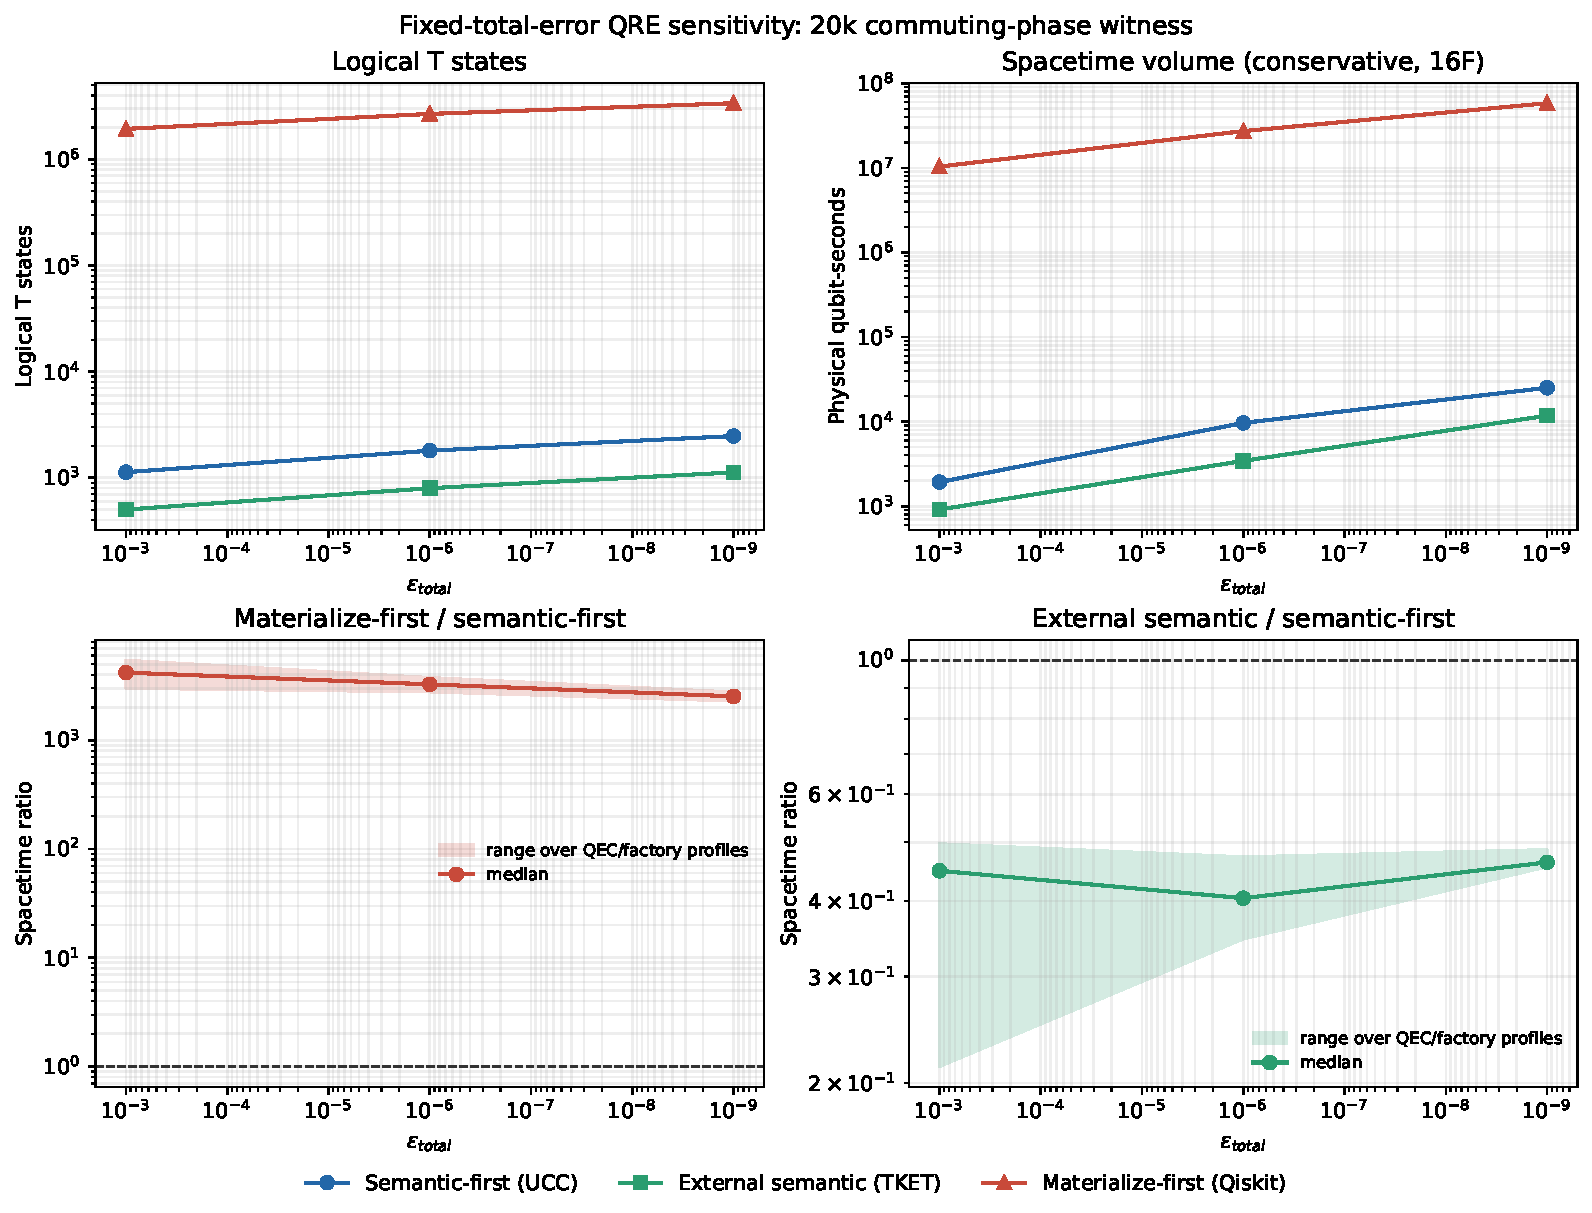
\includegraphics[width=0.48\textwidth]{../../figures/qre_sensitivity.pdf}
\caption{Pareto and sensitivity views generated from the complete W7 parquet
file.  Reversal or disappearance regions would remain visible; none is removed
by filtering.}
\label{supp:fig:w7}
\end{figure}

\section{Natural workloads and complete ablation}
\label{supp:w8}

The natural campaign is a full factorial over the declared families, scales,
seeds, density levels, topologies, and all six binary mechanism toggles.  Each
cell records gates, depth, CX, runtime, RSS, input/output IR bytes, description
bits, dense certificate, and the fixed-error QRE decomposition including data
and factory physical qubits.

\begin{table}[h]
\caption{Matched structured-family result retained without cherry-picking.}
\label{supp:tab:natural}
\centering
\begin{tabular}{lcc}
\toprule
Family & External-minus-authors gates [95\% interval] & Strict success\\
\midrule
% Generated from data/frozen/natural_workload_summary.csv.
controlled\_power\_ladder & 9.0 [5.7, 12.7] & yes \\
diagonal\_hamiltonian & 38.0 [25.9, 51.8] & yes \\
phase\_polynomial\_blocks & -24.3 [-33.8, -16.3] & no \\
qaoa\_ising & 44.7 [33.7, 56.6] & yes \\
qft\_arithmetic & 8.1 [1.9, 13.8] & no \\
qpe\_controlled\_powers & -12.0 [-22.0, -3.0] & yes \\
trotter\_commuting\_blocks & 33.0 [17.6, 48.2] & yes \\
\bottomrule

\end{tabular}
\end{table}

\begin{table}[h]
\caption{All six natural-family gate-count main effects.  Off-minus-on is
positive when enabling the factor reduces gates.}
\label{supp:tab:ablation}
\centering
\begin{tabular}{lrr}
\toprule
Factor & Mean reduction & Bootstrap 95\% interval\\
\midrule
% Generated from data/frozen/natural_ablation_effects.csv.
semantic\_lift & 72.2 & [66.3, 78.1] \\
aggregation & 80.4 & [74.6, 86.4] \\
selector & 0.0 & [0.0, 0.0] \\
cache\_reuse & 0.0 & [0.0, 0.0] \\
preset\_recognizer & 364.9 & [349.8, 380.5] \\
projected\_block\_selection & 0.0 & [0.0, 0.0] \\
\bottomrule

\end{tabular}
\end{table}

The preset recognizer is the largest isolated gate-count contribution.
Semantic lift and aggregation also have positive mean effects.  Selector,
cache/reuse, and projected block selection have zero isolated gate effect in
this reference suite, and this null result is retained.  Both negative
controls have zero all-on-minus-all-off differences for gates, depth, CX,
logical $T$, and spacetime, with no systematic-regression interval.

The line-topology preflight initially found an invalid final-layout
permutation in a candidate router.  That preflight failed its dense certificate
before the frozen campaign.  The router was replaced by an explicit adjacent
CX-SWAP construction that restores identity layout, and the entire campaign
was rerun.  The episode is retained because correctness failures take
precedence over favorable metrics.

\section{Legacy and stress-result registry}
\label{supp:legacy}

The active submission body is the full-length
\path{PaperDraft/ucc_v7_2_prxq_repaired/main.tex}.  The unintegrated 38-page
source is frozen as
\path{PaperDraft/ucc_v7_2_prxq_repaired/legacy_main_v7_2.tex}, and the
superseded nine-page reconstruction is frozen as
\path{PaperDraft/ucc_v7_2_prxq_repaired/short_main_w10.tex}.  Neither frozen
file is the submission source.  The active manuscript retains useful earlier
exact-semantics and stress diagnostics, but labels their provenance and does
not silently mix them with the W3--W9 canonical headline tables.

\small
\begin{longtable}{>{\raggedright\arraybackslash}p{0.20\textwidth}>{\raggedright\arraybackslash}p{0.30\textwidth}>{\raggedright\arraybackslash}p{0.38\textwidth}}
\caption{Disposition of legacy material.}\label{supp:tab:legacy}\\
\toprule
Material & Location & Submission disposition\\
\midrule
\endfirsthead
\toprule
Material & Location & Submission disposition\\
\midrule
\endhead
Exact-semantics four-qubit witnesses & \path{appendix/appendix_C_prxq.tex} & Supplementary context only; not evidence for the $K$-ary asymptotic claim.\\
Finite-range rational CP period & \path{research/rational_witness/} & Retained certificate for the legacy exact-semantics corollary; not a W8 natural result.\\
Packing-width stress run & \path{research/packing_scaling/} & Historical theorem-linked stress evidence; superseded for headline measurements by W3/W4.\\
Width/topology external stress & \path{appendix/appendix_C_prxq.tex} & Status table retained; unsupported/predicate errors are not converted to quality.\\
Historical cut tracing & \path{research/cut_trace/} & Noncanonical after the event-schema revision; W3 event logs are canonical.\\
Earlier matched/natural tables & \path{research/matched_representation/}, \path{research/natural_factorial/} & Archived; W4 and W8 root-level parquet freezes are canonical.\\
Earlier per-rotation proxy QRE & \path{research/fixed_budget_qre/} & Excluded from the main claim; W7 fixed-total-error QRE supersedes it.\\
\bottomrule
\end{longtable}
\normalsize

This separation is deliberate.  It preserves failed and superseded evidence
without allowing duplicate filenames or stale values to support a new claim.

\section{Data lineage and independent-directory reproduction}
\label{supp:w9}

The normalized record key is
\begin{equation*}
 \begin{gathered}
 (\texttt{experiment\_id},\texttt{instance\_id},
  \texttt{representation\_id},\texttt{method\_id},\texttt{seed},\\
  \texttt{backend\_hash},\texttt{tool\_version},
  \texttt{artifact\_commit},\texttt{config\_hash}).
 \end{gathered}
\end{equation*}
The index contains \UnifiedRows\ unique records and retains
\UnifiedPredicateErrors\ predicate-error rows.  CSV/parquet mirror checks,
duplicate-label detection, receipt source hashes, row counts, and orphaned
frozen artifacts are checked by \path{scripts/audit_results.py}.

The clean-room runner copies a minimal artifact to an independent temporary
directory, creates a new venv bound to the locked project packages, and works
only from that directory.  It reruns \CleanTheoryTests\ headline-theorem
tests, independently compiles and densely certifies one matched QAOA/Ising
instance with both reference pipelines, and runs a fixed-error QRE subset that
exercises \CleanGridPairs\ deterministic synthesis pairs.  This is working-
directory isolation, not a claim of binary independence from the host Python
installation.

Every W3--W9 headline experimental number in the main text and this supplement
is a generated macro registered in \path{data/provenance_map.yaml}.  Retained
historical diagnostics keep their original source paths and cannot support a
new headline number unless registered.  The complete machine-readable audit is
\path{data/frozen/data_audit.json}; the clean-room receipt is
\path{data/frozen/clean_room_receipt.json}.

\end{document}
